This section presents the experimental results obtained from applying the methodology described in Section~\ref{sec:method}. The objective is to validate the proposed approaches and analyze the model's behavior under varying conditions. Initially, the computational environment and the hyperparameters used to train the baseline model are described. Next, the impact of the noise-removal stage and different loss-function formulations on predictive performance is investigated. Finally, a comprehensive comparative study across different EfficientNet architectures is conducted, evaluating the trade-off between computational cost and effectiveness.

\subsection{Experimental Environment}

The experiments were conducted on a Linux workstation equipped with an AMD Ryzen 5 5600X processor, 32 GB of DDR4 RAM (3200 MHz), and an NVIDIA GeForce RTX 3060 GPU (12 GB of VRAM), dedicated to accelerating the training of deep learning models. The development was carried out in Python using the PyTorch framework integrated with CUDA 12.8. For histopathological image processing, the OpenSlide library was used to read images and extract patches. The evaluation metrics were computed using scikit-learn, and the visual analyses were generated with Matplotlib.

\subsection{Hyperparameter Configuration}

The initial stage of the experimentation consisted of a grid search to identify the hyperparameter configuration that maximized convergence and generalization of the baseline model, thereby mitigating the risk of overfitting. The explored values and the final selected configuration are summarized in Table~\ref{tab:hiperparametros_gridsearch}. This optimal configuration was established as the standard and kept constant in subsequent experiments to ensure comparability of the results.

The initial learning rate set to $3\times10^{-4}$, operating together with the Adam optimizer, provided the best stability during the minimization of the loss function (BCE). For fine-tuning, unfreezing the last 150 layers of the network yielded the best balance. In addition, a dropout layer with a retention probability of 0.4 proved to be the most effective regularization strategy. The batch size was limited to two samples due to GPU memory constraints. To mitigate fluctuations in gradient updates due to the small batch size, training was configured for up to 50 epochs, using an early stopping criterion with a patience of 7 epochs after no improvement in the validation metric.

To mitigate the limited size of the dataset and improve generalization, data augmentation was applied on-the-fly during training using the Albumentations library. The adopted transformations include random transpositions, horizontal flips, and vertical flips, increasing the variability of the training samples and helping to reduce overfitting.

\begin{table}[htb]
	\centering
	\begin{tabular}{lll}
		\toprule
		\textbf{Parameter} & \textbf{Evaluated values} & \textbf{Selected value} \\
		\midrule
		Learning rate & $3\times10^{-4}$, $3\times10^{-3}$, $1\times10^{-4}$ & $3\times10^{-4}$ \\
		Number of epochs & 50 & 50 \\
		Unfrozen layers (\textit{fine-tuning}) & 100, 150 & 150 \\
		\textit{Dropout} & 0.4, 0.5, 0.6 & 0.4 \\
		Batch size & 2 & 2 \\
		Loss function & BCE & BCE \\
		Optimizer & Adam & Adam \\
		\bottomrule
	\end{tabular}
	\caption{Evaluated hyperparameters and selected configuration for the experiments.}
	\label{tab:hiperparametros_gridsearch}
\end{table}

\subsection{Impact of Noise Filtering and Loss Functions}

With the optimal set of hyperparameters defined, the baseline model was trained using the EfficientNet-B0 architecture and the BCE loss function. This model achieved an accuracy of 0.592 and a Kappa coefficient of 0.826. In the context of ISUP grade classification in prostate biopsies, this Kappa value is considered highly satisfactory and competitive. The medical literature reports considerable interobserver variability in histopathological grading \cite{ozkan2016interobserver, cinar2025assessment}. While experienced uropathologists often achieve Kappa values between 0.43 and 0.68 \cite{ozkan2016interobserver}, more recent evaluations specifically focused on ISUP grades report minimal agreement levels among pathologists, with Kappa values around 0.31 \cite{cinar2025assessment}. Therefore, the obtained baseline demonstrates agreement that considerably exceeds the reported human variability. Furthermore, the results indicate that even with a moderate accuracy (59.2\%), most prediction errors are concentrated between adjacent ISUP grades, minimizing severe clinical penalties.

The entropy-based filtering stage identified a subset of 903 samples, corresponding to the 10\% with the highest uncertainty among the predictions of EfficientNet-B0, B1, B2, and B3 models. The analysis of this subset revealed characteristics indicating great difficulty for the models, including high mean entropy ($0.3851 \pm 0.0638$), high variability in predictions ($1.1188 \pm 0.8943$), and low agreement among the evaluated architectures. It was observed that only 6.2\% of the samples presented consensus among the four models. Additionally, in 58\% of instances classified as \textit{hard samples}, none of the models produced the correct prediction. These findings support the hypothesis that entropy can act as an effective indicator for identifying difficult or inconsistent examples.

Based on this subset of \textit{hard samples}, different scenarios for removing potentially noisy data during training were investigated. The results indicated that partial removal of these samples contributed to improved model performance. As shown in Figure~\ref{fig:acckappa}, removing approximately 20\% of the \textit{hard samples} yielded the best balance between noise reduction and preservation of the training set's diversity, suggesting that moderate filtering may improve the model's generalization capability.

\begin{figure}[H]
	\centering
	
\includegraphics[width=1\linewidth]{images/acc_kappa}
	\caption{Performance under different noise removal thresholds applied to the \textit{hard samples}.}
	\label{fig:acckappa}
\end{figure}

Figure~\ref{fig:maxentropy} presents an example of an image identified by the method as a sample with high prediction uncertainty. When analyzing the models' predictions, the true label is ISUP class 2. However, during inference, EfficientNet-B0 classified it as ISUP 3, whereas EfficientNet-B1, B2, and B3 predicted ISUP 1. Although these discrepancies do not constitute clinically severe errors, the analysis at this stage prioritizes the uncertainty associated with model decisions. For this specific image, the calculated mean entropy value was 0.59, which is considered high. This example illustrates how the method can identify potentially noisy cases; in this particular image, pen annotations are clearly visible. The effectiveness of this filtering strategy becomes more evident when analyzing the results presented in Table~\ref{tab:impacto_loss_expandido}. The application of noise removal increased $\kappa_{\text{quad}}$ from $0.826$ in the baseline model to $0.833$. The impact on accuracy was even more pronounced, increasing from $0.592$ to $0.638$, corresponding to an absolute gain of approximately 4.6 percentage points. These results indicate that removing a fraction of highly uncertain samples improves the model's generalization capability.

\begin{figure}[H]
	\centering
	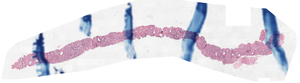
\includegraphics[width=0.7\linewidth]{images/max_entropy}
	\caption{Image identified as noise by the filtering method.}
	\label{fig:maxentropy}
\end{figure}

Replacing the BCE loss function with the ordinal formulation increased the overall model performance to $0.851$, although a slight reduction in accuracy was observed. This result suggests that incorporating the ordinal factor redistributes incorrect predictions, reducing errors between distant classes and concentrating confusions among adjacent classes. In ordinal classification problems, such as the ISUP grading system, this behavior is desirable because discrepancies between neighboring classes have less clinical impact than errors between distant grades. This behavior is shown in Figure~\ref{fig:confusionmatricesbaseline}, which presents normalized confusion matrices for models trained with BCE and the ordinal loss function. It can be seen that the model trained with an ordinal loss concentrates errors primarily between adjacent classes, whereas the BCE-trained model exhibits greater dispersion toward more distant classes.

\begin{figure}[htb]
	\centering
	
\includegraphics[width=1\linewidth]{images/confusion_matrices_baseline}
	\caption{Normalized confusion matrices obtained for the model trained with BCE loss (left) and ordinal loss (right).}
	\label{fig:confusionmatricesbaseline}
\end{figure}

Analyzing the main diagonal of the matrices reveals improvements in ISUP classes 1, 2, and 4, whereas reductions in accuracy were observed for ISUP classes 0, 3, and 5. Moreover, the ordinal loss almost eliminates errors between distant classes. Samples classified as ISUP 0 are no longer classified as ISUP 3, 4, or 5 and are predominantly misclassified as the adjacent class ISUP 1. Conversely, greater dispersion is observed in intermediate classes, particularly ISUP 2 and ISUP 3, reflecting the intrinsic difficulty of distinguishing adjacent histopathological grades. Overall, the results indicate that the use of ordinal loss promotes classification behavior more aligned with the hierarchical nature of the problem, reducing severe discrepancies between classes and favoring confusions between adjacent histopathological grades.

After introducing the ordinal loss, it was observed that dataset imbalance, described in Section~\ref{sub:data}, could be limiting model performance. Therefore, a hybrid loss function that combines ordinal penalization with the focal mechanism was proposed to emphasize more difficult samples and mitigate the effects of class imbalance.

This strategy achieved the best overall performance among the evaluated configurations, reaching a quadratic kappa of 0.857 and an accuracy of 0.669. In addition, it consistently improved classification quality across complementary metrics, achieving a macro F1 Score of 0.612 and macro precision of 0.628 (Table \ref{tab:impacto_loss_expandido}).

\begin{table}[!htb]
	\centering
	\makebox[\textwidth][l]{\hspace{-2.8cm}%
		\resizebox{1.2\textwidth}{!}{%
			\begin{tabular}{lcccccccccccc}
				\toprule
				& \multicolumn{3}{c}{\textbf{Test Quadratic Kappa}} 
				& \multicolumn{3}{c}{\textbf{Test Accuracy (\%)}} 
				& \multicolumn{3}{c}{\textbf{Test F1 Macro}} 
				& \multicolumn{3}{c}{\textbf{Test Precision}} \\
				
				\cmidrule(lr){2-4} \cmidrule(lr){5-7} \cmidrule(lr){8-10} \cmidrule(lr){11-13}
				
				\textbf{Configuration} 
				& \textbf{Result} & \textbf{SD} & \textbf{95\% CI} 
				& \textbf{Result} & \textbf{SD} & \textbf{95\% CI}
				& \textbf{Result} & \textbf{SD} & \textbf{95\% CI}
				& \textbf{Result} & \textbf{SD} & \textbf{95\% CI} \\
				
				\midrule
				
				\quad BCE (baseline) 
				& 0.826 & 0.012 & [0.806; 0.846] 
				& 0.592 & 0.012 & [0.572; 0.612]
				& 0.537 & 0.013 & [0.516; 0.558]
				& 0.551 & 0.013 & [0.530; 0.572] \\
				
				\quad BCE + Noise Removal 
				& 0.833 & 0.013 & [0.812; 0.853] 
				& 0.638 & 0.116 & [0.619; 0.657]
				& 0.572 & 0.013 & [0.553; 0.594]
				& 0.584 & 0.013 & [0.563; 0.606] \\
				
				\quad Ordinal Loss 
				& 0.851 & \textbf{0.009} & [0.833; 0.869] 
				& 0.608 & 0.126 & [0.587; 0.628]
				& 0.559 & 0.014 & [0.537; 0.581]
				& 0.585 & 0.013 & [0.563; 0.606] \\
				
				\quad \textbf{Ordinal + Focal (Hybrid)} 
				& \textbf{0.857} & 0.011 & [0.833; 0.876] 
				& \textbf{0.669} & 0.011 & [0.635; 0.683]
				& \textbf{0.612} & 0.013 & [0.587; 0.636]
				& \textbf{0.628} & 0.013 & [0.603; 0.653] \\
				
				\bottomrule
			\end{tabular}%
	}}
	\caption{Incremental impact of the proposed strategies on the performance of EfficientNet-B0}
	\label{tab:impacto_loss_expandido}
\end{table}

The learning dynamics illustrated in Figure \ref{fig:training_curves} provide important insights into the behavior of each training strategy. The baseline model (BCE) exhibits clear overfitting: while the training loss decreases rapidly, the validation loss steadily increases after the first epochs. This divergence is reflected in the validation QWKappa, which improves initially but then fluctuates and stabilizes at a lower level, indicating limited generalization.

The application of entropy-based noise removal partially mitigates this issue. Although the validation loss still shows an increasing trend, its rate of increase is less abrupt than the baseline. This results in a more stable improvement in QWKappa, which reaches higher values than BCE, suggesting that removing highly uncertain samples improves the quality of the training signal, even if overfitting is not fully eliminated.

The introduction of the Ordinal Loss leads to a noticeable change in training dynamics. Both training and validation losses become more stable, with a smaller gap between them, indicating better generalization. This is reflected in the smoother, more consistent increase in QWKappa, which reaches competitive values while exhibiting fewer fluctuations than previous approaches.

Finally, the Hybrid approach (Ordinal + Focal) demonstrates the most stable convergence behavior. The validation loss remains relatively stable throughout training, despite some oscillations, and the gap between the training and validation losses is smaller than with BCE-based methods. The QWKappa curve shows a consistent upward trend with reduced variability, achieving the highest and most stable performance among all configurations. These results suggest that combining ordinal learning with focal weighting improves training stability and enhances the model’s ability to handle difficult and imbalanced samples.

\begin{figure}[htbp]
	\centering
	\makebox[\linewidth][l]{%
		\hspace*{-2.8cm}
		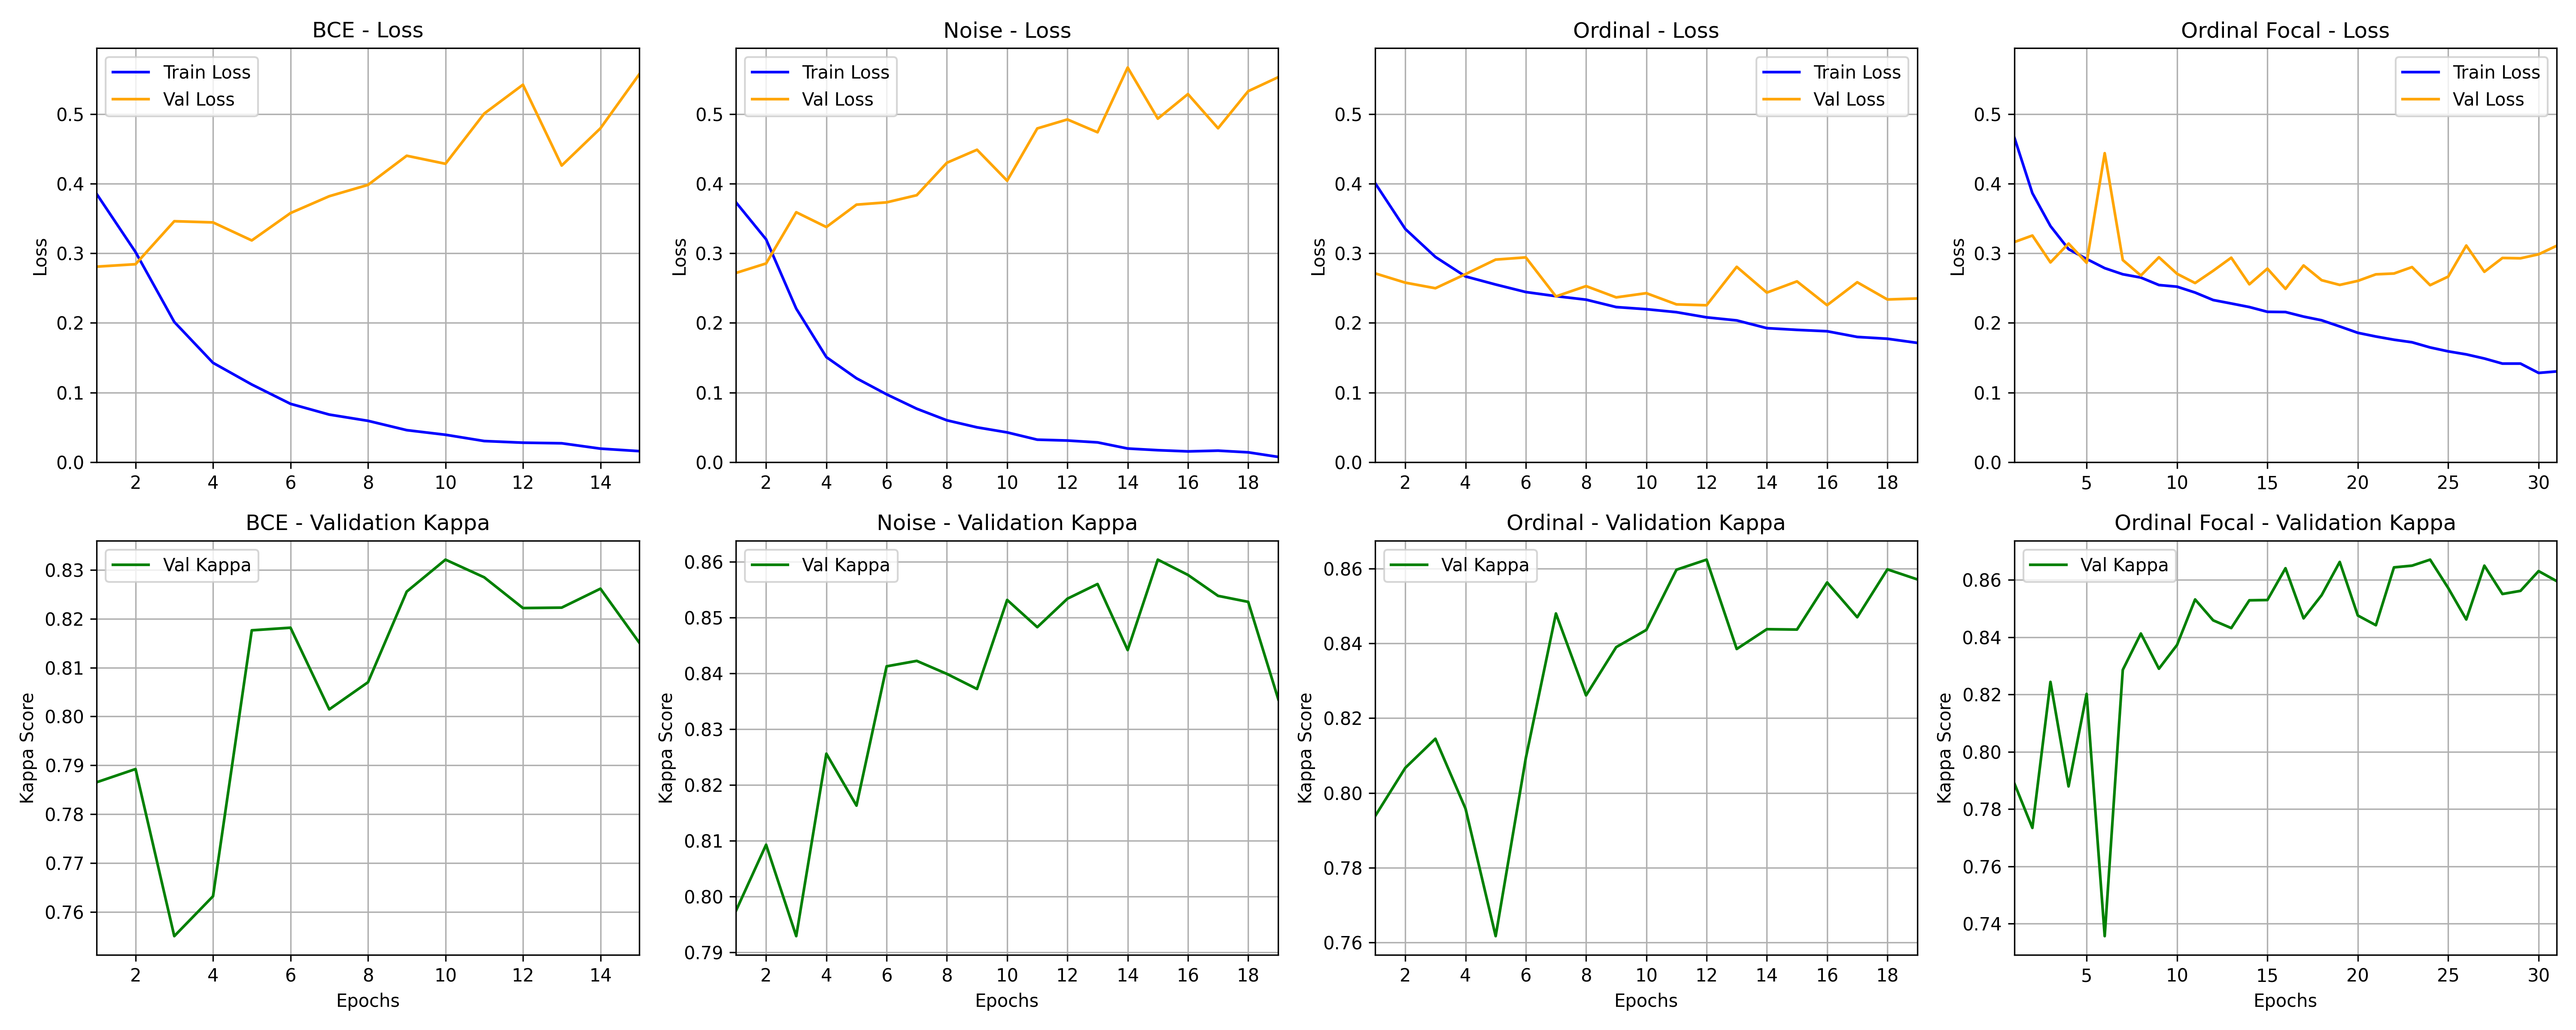
\includegraphics[width=1.2\linewidth]{images/plot_loss_kappa_4models.png}%
	}
	\caption{Loss and kappa curves during training and validation}
	\label{fig:training_curves}
\end{figure}


The analysis of the confusion matrices presented in Figure~\ref{fig:cm_ordinal_focal} reveals consistent improvements when using the ordinal focal loss. The model trained only with ordinal loss exhibits greater dispersion across intermediate classes, particularly for ISUP class 3, whose accuracy was $0.365$, with a considerable portion of samples being misclassified as ISUP 2 ($0.303$) and ISUP 4 ($0.212$). In contrast, the hybrid model shows greater concentration of predictions along the main diagonal, indicating improved discriminative capability. Relevant improvements are observed across several classes, including ISUP 0 ($0.857$ vs.\ $0.711$), ISUP 3 ($0.492$ vs.\ $0.365$), and ISUP 4 ($0.652$ vs.\ $0.498$). In addition, a reduction in confusion between intermediate classes is observed, particularly between ISUP 2 and ISUP 3, suggesting greater separability between these histopathological grades.

Another important aspect is the improved distinction between high-grade classes. In the ordinal model, a significant proportion of ISUP 5 samples were classified as ISUP 4 ($0.342$). Although this confusion remains in the hybrid model ($0.380$), an increase in accuracy for ISUP 4 ($0.652$ vs.\ $0.498$) is observed, indicating improved discrimination between higher grades.

\begin{figure}[!htb]
	\centering
	\subfloat[\centering Ordinal]{
		
\includegraphics[width=0.47\textwidth]{images/cm_ordinal.png} 
		\label{subfig:ordinal}
	}%
	\hspace{0.2cm}
	\subfloat[\centering Ordinal Focal]{
		
\includegraphics[width=0.47\textwidth]{images/cm_ordinal_focal.png} 
		\label{subfig:ordinal_focal}
	}%
	\caption{Normalized confusion matrices for models trained with ordinal loss and ordinal focal loss.}
	\label{fig:cm_ordinal_focal}
\end{figure}

\subsection{Comparison Among EfficientNet Architectures}

The experimental configuration defined for EfficientNet-B0 was also applied to EfficientNet-B3 and EfficientNet-B7, including the proposed hybrid loss function. The objective was to evaluate whether deeper architectures could provide additional performance gains. 

The results, presented in Table~\ref{tab:comparacao_arquiteturas}, indicate that EfficientNet-B0 achieved the best overall performance across all evaluated metrics, including quadratic kappa, accuracy, macro F1-score, and macro precision. In particular, EfficientNet-B0 outperformed the deeper variants not only in terms of ordinal consistency (kappa) and overall correctness (accuracy), but also in balanced classification performance, as reflected by the highest F1 Macro and Precision values.

\begin{table}[!htb]
	\centering
	\makebox[\textwidth][l]{\hspace{-2.8cm}%
		\resizebox{1.2\textwidth}{!}{%
			\begin{tabular}{lcccccccccccc}
				\toprule
				& \multicolumn{3}{c}{\textbf{Test Quadratic Kappa}} 
				& \multicolumn{3}{c}{\textbf{Test Accuracy (\%)}} 
				& \multicolumn{3}{c}{\textbf{Test F1 Macro}} 
				& \multicolumn{3}{c}{\textbf{Test Precision}} \\
				
				\cmidrule(lr){2-4} \cmidrule(lr){5-7} \cmidrule(lr){8-10} \cmidrule(lr){11-13}
				
				\textbf{Architecture} 
				& \textbf{Result} & \textbf{SD} & \textbf{95\% CI} 
				& \textbf{Result} & \textbf{SD} & \textbf{95\% CI}
				& \textbf{Result} & \textbf{SD} & \textbf{95\% CI}
				& \textbf{Result} & \textbf{SD} & \textbf{95\% CI} \\
				
				\midrule
				
				EfficientNet-B0 
				& \textbf{0.857} & 0.011 & [0.833; 0.876] 
				& \textbf{0.669} & 0.011 & [0.635; 0.683]
				& \textbf{0.612} & 0.013 & [0.587; 0.636]
				& \textbf{0.628} & 0.013 & [0.603; 0.653] \\
				
				EfficientNet-B3 
				& 0.849 & 0.013 & [0.824; 0.870] 
				& 0.661 & 0.014 & [0.634; 0.685]
				& 0.555 & 0.013 & [0.532; 0.576]
				& 0.605 & 0.012 & [0.585; 0.624] \\
				
				EfficientNet-B7 
				& 0.842 & 0.015 & [0.815; 0.866] 
				& 0.654 & 0.016 & [0.628; 0.678]
				& 0.556 & 0.013 & [0.530; 0.579]
				& 0.561 & 0.013 & [0.536; 0.586] \\
				
				\bottomrule
			\end{tabular}%
	}}
	\caption{Performance comparison among EfficientNet architectures using the proposed experimental configuration.}
	\label{tab:comparacao_arquiteturas}
\end{table}

The results indicate that the hyperparameters optimized for EfficientNet-B0 do not generalize uniformly to deeper variants of the architecture. Since the same configuration, including the learning rate and early stopping strategy, was directly applied to the B3 and B7 models, distinct training and generalization behaviors were observed. As shown in Figure~\ref{fig:plotlosskappa}, The B3 model exhibited clear signs of overfitting, characterized by a continuous decrease in training loss alongside a progressive increase in validation loss. Nevertheless, it achieved performance comparable to B0 in terms of kappa, suggesting that its higher representational capacity partially compensated for the lack of adequate regularization, allowing it to better fit the underlying signal despite reduced generalization.
In contrast, the B7 model showed no signs of overfitting but also did not achieve superior performance. Instead, it displayed rapid convergence and early stabilization of the metrics, indicating difficulty in fully leveraging its higher capacity. This behavior suggests undertraining, where hyperparameters calibrated for a smaller architecture, particularly the learning rate and early stopping criterion, limited the optimization and prevented the model from reaching its full potential.
Overall, these findings reinforce the idea that hyperparameters do not scale linearly with model depth, highlighting the need for architecture-specific tuning, especially for learning rate, regularization strategies, and the number of training epochs.

\begin{figure}[htbp]
	\centering
	\makebox[\linewidth][l]{%
		\hspace*{-5cm}
		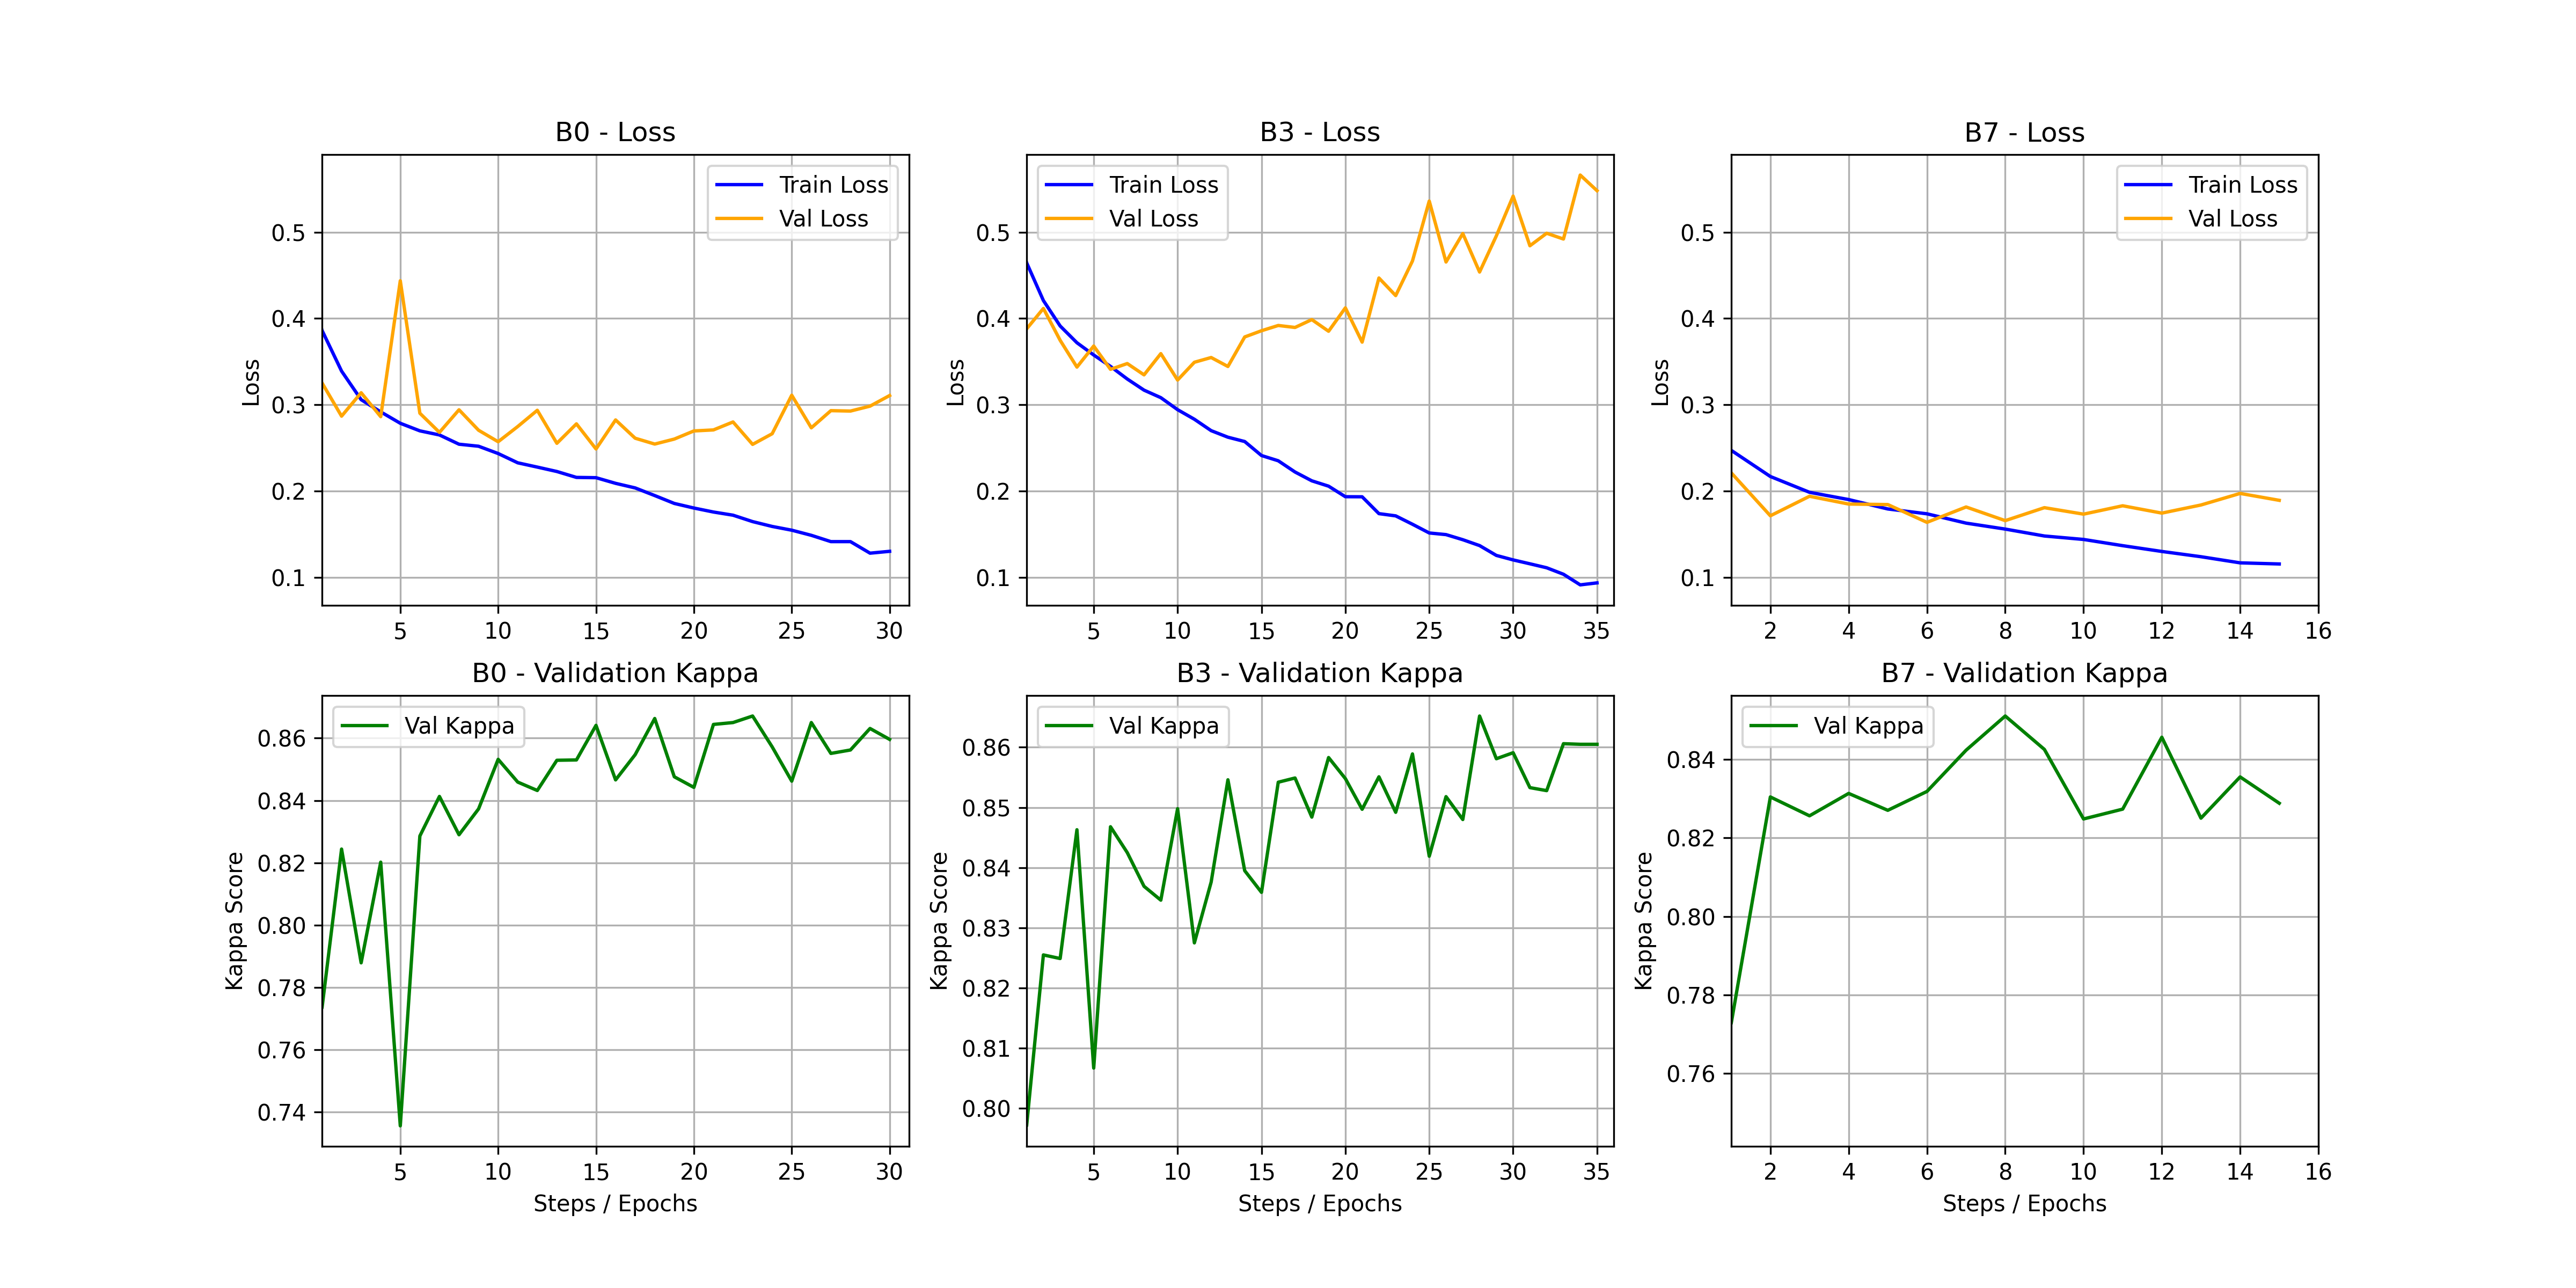
\includegraphics[width=1.5\linewidth]{images/plot_loss_kappa}%
	}
	\caption{Loss and kappa curves during training and validation}
	\label{fig:plotlosskappa}
\end{figure}

